%%%%%%%%%%%%%%%%%%%%%%%%%%%%%%%%%%%%%%%%%%%%%%%%%%%%%%%%%%%%%%%%%%%%%%
% CS1231S Midterms Cheatsheet
% Author: San Diego John Michael Bautista
%%%%%%%%%%%%%%%%%%%%%%%%%%%%%%%%%%%%%%%%%%%%%%%%%%%%%%%%%%%%%%%%%%%%%%

\documentclass[10pt,landscape]{article}
\usepackage{amssymb,amsmath,amsthm,amsfonts}
\usepackage[mathscr]{euscript}
\usepackage{multicol,multirow}
\usepackage{calc}
\usepackage{ifthen}
\usepackage[landscape]{geometry}
\usepackage[colorlinks=true,citecolor=blue,linkcolor=blue]{hyperref}
\usepackage{mdframed}
\usepackage{graphicx}
\graphicspath{{./images/}}

\ifthenelse{\lengthtest { \paperwidth = 11in}}
{ \geometry{top=.5in,left=.5in,right=.5in,bottom=.5in} }
{\ifthenelse{ \lengthtest{ \paperwidth = 297mm}}
    {\geometry{top=1cm,left=1cm,right=1cm,bottom=1cm} }
    {\geometry{top=1cm,left=1cm,right=1cm,bottom=1cm} }
}
\pagestyle{empty}
\makeatletter
\renewcommand{\section}{\@startsection{section}{1}{0mm}%
    {-1ex plus -.5ex minus -.2ex}%
    {0.5ex plus .2ex}%x
    {\normalfont\large\bfseries}}
\renewcommand{\subsection}{\@startsection{subsection}{2}{0mm}%
    {-1explus -.5ex minus -.2ex}%
    {0.5ex plus .2ex}%
    {\normalfont\normalsize\bfseries}}
\renewcommand{\subsubsection}{\@startsection{subsubsection}{3}{0mm}%
    {-1ex plus -.5ex minus -.2ex}%
    {1ex plus .2ex}%
    {\normalfont\small\bfseries}}
\makeatother
\setcounter{secnumdepth}{0}
\setlength{\parindent}{0pt}
\setlength{\parskip}{0pt plus 0.5ex}

% -----------------------------------------------------------------------

\title{CS1231S Midterms CheatSheet}

\begin{document}

\raggedright
\footnotesize

\begin{center}
    \Large{\textbf{CS1231S Midterms Cheatsheet}} \\
    by @jmsandiegoo
\end{center}
\begin{multicols}{3}
    % \setlength{\premulticols}{1pt}
    % \setlength{\postmulticols}{1pt}
    % \setlength{\multicolsep}{1pt}
    \setlength{\columnsep}{2pt}

    % -----------------------------------------------------------------------
    % 1. Proofs
    % -----------------------------------------------------------------------

    \begin{mdframed}
        \section{1. Proofs}
    \end{mdframed}

    \subsection{Number System Sets}
    $\mathbb{N}$: Natural numbers $\{0,1,2,...\}$ ($\mathbb{Z}_{\geq 0}$) \\
    $\mathbb{Z}$: Integers $\{3,-100,3^5,...\}$ \\
    $\mathbb{Q}$: Rational Numbers $\{\frac{1}{2},-23,8.6,\frac{-37}{5},...\}$\\
    $\mathbb{R}$: Real Numbers $\{-1,\pi,\sqrt[]{2},4.5,...\}$\\
    \textit{* 0 is neither negative or positive} \\
    \textit{* ${\mathbb{Z}^{+/-}}$ set of all positive or negative integers} \\
    \subsection{Terminologies}
    \textbf{Axiom/Postulate}: A statement assumed to be true w/o proof. Basic building blocks of theorems \\
    \textbf{Theorem}: A mathematical statement proved using rigorous mathematical reasoning. Major / important result. \\
    \textbf{Lemma}: A small theorem minor result to help prove a theorem. \\
    \textbf{Corollary}: Simple deduction from Theorem. \\
    \textbf{Conjecture}: A statement believed to be true, but no proof yet. \\

    \subsection*{Basic Properties of Integers}
    \textbf{Closure}: Closed under $+ / \times / -$\\
    $x + y \in \mathbb{Z}$ and $xy \in \mathbb{Z}$ \\
    \textbf{Commutativity}: Commutative under $+ / \times$ \\
    $x + y = y + x$ and $xy = yx$ \\
    \textbf{Associativity}: Associative under $+ / \times$ \\
    $x + y + z = (x + y) + z = x + (y + z)$ and $xyz = (xy)z = x(yz)$ \\
    \textbf{Distributivity}: \\
    $x(y+z) = xy + xz$ \\
    \textbf{Trichotomy}: Exactly one of the following is true \\
    $x=y$ or $x<y$ or $x>y$

    \subsection*{Definitions of Number}
    \subsubsection {Even and Odd Integers}
    Let $n \in \mathbb{Z}$ \\
    n is even $\leftrightarrow$ $\exists k \in \mathbb{Z}$ $n = 2k$ \\
    n is odd $\leftrightarrow$ $\exists k \in \mathbb{Z}$ $n = 2k + 1$s
    \subsubsection {Divisibility}
    Let $d, n \in \mathbb{Z} \; \land d \neq 0$\\
    $d | n \leftrightarrow \exists k \in \mathbb{Z} \; n = dk$ \\
    \textit{* d divides n}
    \subsubsection{Prime / Composite}
    \subsubsection{Congruence}
    Let $a, b \in \mathbb{Z}$ and $n \in \mathbb{Z}^+$:\\
    $a \equiv b (mod n) \leftrightarrow n | (a-b)$ \\
    \textit{* forms equivalence relation}

    \subsubsection{Rationality / Lowest Term Fraction}
    $r$ is rational $\leftrightarrow$ $\exists a, b \in \mathbb{Z}\; r=\frac{a}{b} \land b \neq 0$ \\
    \textit{* it is lowest term fraction if largest integer that divides $a \land b$ in $\frac{a}{b}$ is 1 (prime numbers)}
    \subsection{Methods of Proof}
    \begin{enumerate}
        \item \textbf{Proof by Construction}: usually proves an existential statement by explicitly finding / constructing a value that satisfies the properties stated.
        \item \textbf{Proof by Counter Example}: Finding a specific example that shows statement is not always true.
        \item \textbf{Proof by Exhaustion}: Prove by showing each cases is true. Suitable for finite cases.
        \item \textbf{Proof by Deduction}: Form of direct proof usually makes use of definitions. Good for universal statements and infinite cases.
        \item \textbf{Proof by Contradiction}: Negating the original statement and trying to arrive at a contradiction making the negation to be false.
    \end{enumerate}
    \begin{mdframed}
        \section{2. Compound Statements}
    \end{mdframed}
    \textbf{Definition 2.1.1 (Statement)} \\
    A statement / proposition is a sentence that is true or false, but not both \\
    \textbf{Definition 2.1.2 (Negation)} \\
    If p is a statement variable, negation is "not p $(\sim p)$"
    \textbf{Definition 2.1.3 (Conjunction)} \\
    "p and q ($p \land q$)" \\
    \textbf{Definition 2.1.4 (Disjunction)} \\
    "p or q ($p \lor q$)" \\
    \textit{* $\sim$ performed first, then $\land$, $\lor$ coequal in order of operation} \\
    \textbf{Definition 2.1.5 (Statement / Propositional Form)}
    A statement / propositional form is an expression of statement variables and logical connectives that becomes a statement when actual statements are substituted \\
    \textbf{Definition 2.1.6 (Logical Equivalence}) \\
    $P \equiv Q \leftrightarrow$ both have identical truth values \\
    \textit{* Use truth table / counter example to prove non-equivalence} \\
    \textbf{Definition 2.1.7 (Tautology)} \\
    Statement that is always true (tautological statement) \\
    \textbf{Definition 2.1.8 (Contradiction)} \\
    Statement that is always false (contradictory statement) \\
    \subsection{Conditional Statements}
    \textbf{Definition 2.2.1 (Conditional)} \\
    "if p then q" or "p implies q" \\
    $p\;(hypo / antedecent) \rightarrow q\;(conclusion / consequent)$ \\
    \textit{* only false when p is true and q is false} \\
    \textit{* performed last with $\sim, \land, \lor$} \\
    \textbf{Vacuously true}: hypothesis is false \\
    \textbf{Implication}: $\sim p \lor q$ \\
    \textbf{Negation}: $p\; \land \sim q$ \\
    \textbf{Definition 2.2.2 (Contrapositive)} \\
    "$p \rightarrow q \equiv \sim q \rightarrow \; \sim p$" \\
    \textbf{Definition 2.2.3 (Converse)} \\
    "$q \rightarrow p$" \\
    \textbf{Definition 2.2.4 (Inverse)} \\
    "$\sim p \rightarrow \; \sim q"$ \\
    \textit{* Inverse $\equiv$ Converse} \\
    \textbf{Definition 2.2.5 (Only If)} \\
    p can only take place only if q takes place. "$\sim q \rightarrow \; \sim p$"
    \textbf{Definition 2.2.6 (Biconditional $\leftrightarrow$ )} \\
    "$p \leftrightarrow q$" implication but both ways. True when p and q has same value false otherwise. \\
    \textit{* Proving it needs to show both direction (Proof by cases $\rightarrow$ and $\leftarrow$)} \\
    \textit{* Coequal with Conditional operator} \\
    \textbf{Definition 2.2.7 (Necessary / Sufficient)} \\
    "$p \rightarrow q$" means p is sufficient to guarantee occurrence of q.
    "$\sim p \rightarrow \sim q$" means if p does not occur, q does not either. Necessary for p to occur when q occurs \\
    \subsection{Arguments}
    \textbf{Definition 2.3.1 (Argument)} \\
    \begin{align}
        p \rightarrow q \tag{premise} \\
        p \tag{premise}               \\
        \bullet \hspace{0.3cm} q \tag{conclusion}
    \end{align}
    \textbf{Valid}: All premises (critical rows) and conclusion are true.
    \textbf{Syllogism}: Argument form consisting of two premises and a conclusion.
    \subsection{Rules of inference}
    \textbf{Modus Ponens} \\
    \begin{align}
        p \rightarrow q \tag{premise} \\
        p \tag{premise}               \\
        \bullet \hspace{0.3cm} q \tag{conclusion}
    \end{align}
    \textbf{Modus Tollens} \\
    \begin{align}
        p \rightarrow q \tag{premise} \\
        \sim q \tag{premise}          \\
        \bullet \hspace{0.3cm} \sim p \tag{conclusion}
    \end{align}
    \textbf{Generalization} \\
    \begin{align}
        p \tag{premise} \\
        \bullet \hspace{0.3cm} p \lor q \tag{conclusion}
    \end{align}
    \textbf{Specialization} \\
    \begin{align}
        p \land q \tag{premise} \\
        \bullet \hspace{0.3cm} p \tag{conclusion}
    \end{align}
    \textbf{Elimination} \\
    \begin{align}
        p \lor q \tag{premise} \\
        \sim q \tag{premise}   \\
        \bullet \hspace{0.3cm} p \tag{conclusion}
    \end{align}
    \textbf{Transitivity} \\
    \begin{align}
        p \rightarrow q \tag{premise} \\
        q \rightarrow r \tag{premise} \\
        \bullet \hspace{0.3cm} p \rightarrow r \tag{conclusion}
    \end{align}
    \textbf{Div into Cases} \\
    \begin{align}
        p \lor q \tag{premise}        \\
        p \rightarrow r \tag{premise} \\
        q \rightarrow r \tag{premise} \\
        \bullet \hspace{0.3cm} r \tag{conclusion}
    \end{align}
    \textbf{Contradiction} \\
    \begin{align}
        \sim p \rightarrow false \tag{premise} \\
        \bullet \hspace{0.3cm} p \tag{conclusion}
    \end{align}
    \subsection{Fallacies}
    \begin{enumerate}
        \item Converse
        \item Inverse
        \item False Premise
    \end{enumerate}
    \textbf{Definition 2.3.2 (Sound / Unsound Arguments)} \\
    Sound $\leftrightarrow$ if it is valid and premises are true \\
    Unsound $\leftrightarrow$ $\sim$ Sound

    \begin{mdframed}
        \section{3. Quantified Statement}
    \end{mdframed}
    \textbf{Definition 3.1.1 (Predicate)}: is a sentence that contains a finite number of variables that becomes a statement when values are substituted \\
    \textbf{Definition 3.1.2 (Truth Set)}: set of all elements in Domain of P(x) such that P(x) is true \\
    \textbf{Definition 3.1.3 (Universal Statement $\forall$)}: "$\forall x \in D, Q(x)$" \\
    \textit{* true $\leftrightarrow$ Q(x) $\equiv$ True for every x in D} \\
    \textit{* false $\leftrightarrow$ Q(x) $\equiv$ False for at least one x in D (counter-example)} \\
    \textbf{Definition 3.1.4 (Existential Statement $\exists$)}: "$\exists x \in D, Q(x)$" \\
    \textit{* true $\leftrightarrow$ Q(x) $\equiv$ True for at least one x in D} \\
    \textit{* false $\leftrightarrow$ Q(x) $\equiv$ False for all x in D (counter-example)} \\
    \textit{* $\exists!$: there exists a unique / one and only one} \\
    \textbf{Theorem 3.2.1 Negation of a Universal Statement}: "$\sim (\forall x \in D, P(x)) \equiv \exists x \in D, \sim P(x)$" \\
    \textbf{Theorem 3.2.2 Negation of a Existential Statement}: "$\sim (\exists x \in D, P(x)) \equiv \forall x \in D, \sim P(x) $" \\
    \textbf{Definition 3.2.1 (Contrapositive, converse, inverse)}: \\
    Given "$\forall x \in D (P(x) \rightarrow Q(x))$"
    \begin{enumerate}
        \item Contrapositive: "$\forall x \in D (\sim Q(x) \rightarrow \sim P(x))$"
        \item Converse: "$\forall x \in D (Q(x) \rightarrow P(x))$"
        \item Inverse: "$\forall x \in D (\sim P(x) \rightarrow \sim Q(x))$"
    \end{enumerate}

    \begin{mdframed}
        \section{5. Set Theory}
    \end{mdframed}
    \subsection{Set notations:}
    \begin{itemize}
        \item \textbf{Set-Roster Notation}: $\{ 1, 2, 3, ...\}$
        \item \textbf{Set-Builder Notation}: $\{ x \in U : P(x) \}$
        \item \textbf{Replacement Notation}: $\{ t(x) : x \in U \}$
    \end{itemize}
    \textit{* $:$ or $|$} \\
    \textit{* Order and duplicates do not matter} \\
    \textbf{Definitions 5.1.2 (Subset, Proper Susbset Empty Set, Singleton):} \\
    \textbf{Subset $\subseteq$}: $A \subseteq B \leftrightarrow \forall x (x \in A \rightarrow x \in B)$ \\
    \textbf{Proper Subset $\subsetneq $}: $A \subsetneq B \leftrightarrow A \subseteq B \land A \neq B$ \\
    \textbf{Not a subset $ \not\subseteq$}: $A \not\subset B \leftrightarrow \exists x (x \in A \land x \not\in B)$ \\
    \textbf{Theorem 6.2.4 (Empty set subset of every set)} \\
    $\emptyset \subseteq A$ (A is any set) \\
    \textbf{Singleton:} a set with single element \\
    \textbf{Definition 5.1.3 (Ordered Pair)} \\
    Form of $(x, y)$. Equality: $(a, b) = (c, d) \leftrightarrow (a = c) \land (b = d)$ \\
    \textbf{Definition 5.1.4 (Cartesian Product)} \\
    $A \times B = \{(a, b) : a \in A \land b \in B\}$ \\
    \textbf{Definition 5.1.5 (Set Equality)} \\
    $A = B \leftrightarrow A \subseteq B \land B \subseteq A$ \\
    $A = B \leftrightarrow \forall x (x \in A \leftrightarrow x \in B)$ \\
    \textit{* provide A $\subseteq$ B then prove B $\subseteq$ A} \\
    \textbf{Union $\cup$} \\
    $A \cup B = \{ x \in U : x \in A \lor x \in B \}$ \\
    \textbf{Intersection $\cap$} \\
    $A \cap B = \{ x \in U : x \in A \land x \in B \}$ \\
    \textbf{Difference / Relative Complement $- \setminus$} \\
    $B \setminus A = \{ x \in U : x \in B \land x \notin A \}$ \\
    \textbf{Complement $\bar{A}$} \\
    $\bar{A} = \{ x \in U : x \notin A \}$ \\
    \textbf{Definition 5.1.8 (Partition of Sets)} \\
    For all $i, j, ... = 1, 2, 3$ \\
    $A_i \cap A_j = \emptyset | i \neq j$ \\
    \textbf{Theorem 4.4.1 (The Quotient-Remainder Theorem)} \\
    For any integer n and positive integer d, there is a unique q and r such that:\\
    $n = dq + r \; | \; (0 \leq r < d)$ \\
    \textbf{Definition 5.1.9 (Power Set):} \\
    Given $A = \{ x, y \}$,
    $\mathcal{P}(A)$ is the set of all subsets of A \\
    $\mathcal{P}(A) = \{ \emptyset, \{ x \}, \{ y \}, \{ x, y \} \}$ \\
    \textit{* $2^n$ elements for power set} \\
    \textbf{Theorem 6.3.1 (Power Set No. of Elements)} \\
    $|\mathcal{P}(A)| = 2^{|A|}$ \\
    \textbf{Theorem 6.2.1 Some Subset Relations (Property of Sets)} \\
    \begin{enumerate}
        \item Inclusion of Intersection: For all sets A and B \\
              (a)$A \cap B \subseteq A$ (b) $A \cap B \subseteq B$
        \item Inclusion in Union: For all sets A and B \\
              (a)$A \subseteq A \cup B$ (b)$B \subseteq A \cup B$
        \item Transitive Property of Subsets: For all sets A, B and C \\
              $A \subseteq B \land B \subseteq C \rightarrow A \subseteq C$
    \end{enumerate}
    \begin{mdframed}
        \section{6. Relations}
    \end{mdframed}
    \subsection{Relations}
    \textbf{Defintion 6.1.1 (Relation $R$):} \\
    $x R y \leftrightarrow (x, y) \in R$ \\
    \textit{* $R \subseteq A \times B$} \\
    \textbf{Domain $Dom(R)$:} $\{ a \in A : a R b \; \exists b \in B\}$ \\
    \textbf{Co-Domain $coDom(R)$:} set $B$ \\
    \textbf{Range $Range(R)$:} $\{ b \in B : a R b \; \exists a \in A\}$ \\
    \textbf{Definition 6.1.2 (Inverse of a Relation $R^{-1}$):} \\
    Given R from A to B. Inverse: \\
    $R^{-1} = \{(y,x) \in B \times A : (x, y) \in R \}$ \\
    \textbf{Definition 6.1.4 (Composition of Relations):} \\
    Given sets A, B and C. $R \subseteq A \times B$ $S \subseteq B \times C$: \\
    $\forall x \in A, \forall x \in C (x S \circ R z \leftrightarrow (\exists \in B (x R y \land y R z)))$ \\
    \textit{* 2nd relation first} \\
    \textbf{Proposition: Composition is Associative:} \\
    $T \circ (S \circ R) = (T \circ S) \circ R = T \circ S \circ R$ \\
    \textbf{Proposition: Inverse of Composition} \\
    $(S \circ R)^{-1} = R^{-1} \circ S^{-1}$ \\
    \textbf{Definition: (Relexivity, Symmetry, Transitivity):} \\
    \begin{enumerate}
        \item Reflexive: $R$ is reflexive $\leftrightarrow \forall x \in A (x R X)$
        \item Symmetric: $R$ is Symmetric $\leftrightarrow \forall x, y \in A (x R y \rightarrow y R x)$
        \item Transitive: $R$ is Transitive $\leftrightarrow \forall x, y, z \in A (x R y \land y R x \rightarrow x R z)$
    \end{enumerate}
    \textbf{Transitive Closure} \\
    $R^t$ is a transitive closure when it adds least no. of ordered pairs to ensure transitivity: \\
    \begin{enumerate}
        \item $R^t$ is transitive
        \item $R \subseteq R^t$
        \item If $S$ is another transitive relation, $R^t \subseteq S$
    \end{enumerate}

    \subsection{Equivalence Relation}
    \textbf{Definition (Partition $\mathscr{C}$):} \\
    $\mathscr{C}$ is a partition of set A if the following holds:
    \begin{enumerate}
        \item $\forall S \in \mathscr{C}, (\emptyset \neq S \land S \subseteq A)$ \\
              \textit{* $S$ is a subset of $A$}
        \item $\forall x \in A \; \exists S \in \mathscr{C} (x \in S) \land
                  \forall x \; \exists S_1, S_2 \in \mathscr{C} (x \in S_1 \land x \in S_2 \rightarrow S_1 = S_2)$ \\
              \textit{* Every element in A is in exactly one element of $\mathscr{C}$}
        \item Shorter Ver.: $\forall x \in A \exists! S \in \mathscr{C} (x \in S)$
    \end{enumerate}
    \textbf{Theorem 8.3.1 (Relation Induced by a Partition):} \\
    R induced by partition is reflexive, symmetric and transitives \\
    \textit{* same component as relation} \\
    \textbf{Definition 6.3.2 (Equivalence Relation $\sim$):} \\
    $R$ is an equiv relation $\leftrightarrow$ R is reflexive, symmetric, transitive \\
    \textit{* Prove by each cases of reflexive, symmetric, transitive} \\
    \textbf{Definition 6.3.3 (Equivalence Class $[a]_\sim$):} \\
    $[a]_\sim = \{ x \in A : a \sim x \}$ \\
    \textit{* The set consisting of elements related to a} \\
    $\forall a \in A (x \in [a]_\sim \leftrightarrow a \sim x)$ \\
    \textbf{Lemma Rel.1 Equivalence Class} \\
    $x \sim y \equiv [x] = [y] \equiv [x] \cap [y] \neq \emptyset$ \\
    \textbf{Definition 6.3.5 (Set of Equivalent Classes):} \\
    $A /\sim = \{ [x]_\sim : x \in A \}$ \\
    \textit{* set of all equivalence classes} \\
    \textbf{Theorem 8.3.4 (Partiton Induced By Equiv Relation):} \\
    Partition formed by distinct equivalence classes formed by R on set A \\
    \textbf{Theorem Rel.2 ($A /\sim$ is a partition of $A$):} \\
    Partition formed by distinct equivalence classes formed by R on set A \\
    \textbf{Proposition ${\sim}_n$: } Congruence-mod $n$ is an equivalence relation on $\mathbb{Z}$ for every $n \in \mathbb{Z}^+$ \\
    \textit{* Partition into {Theorem 4.4.1 Quotient-Remainder Theorem}} \\
    \subsection{Partial Order Relations}
    \textbf{Definition 3.4.1 (Antisymmetry):} \\
    $R$ is antisymmetric $\leftrightarrow \forall x,y \in A (x R y \land y R x \rightarrow x = y)$ \\
    \textbf{Defintion 6.4.2 (Partial Order Relation $\preceq$)} \\
    $R$ is a partial order relation $\leftrightarrow$ R is reflexive, antisymmetric, transitive \textit{* e.g $(\leq / \subseteq)$} \\
    \textbf{Defintion (Partial Order Set $(A, R)$):} \\
    Given partial order relation $R$ on set $A$, $A$ is the poset \\
    \textit{* divides relation is partial order} \\
    \textbf{Hasse Diagram} \\
    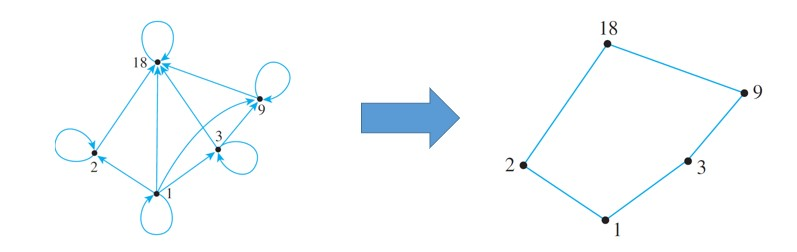
\includegraphics[width=\linewidth]{hasse_diagram}
    \textbf{Definition Comparability:} \\
    $\forall a, b \in A$ ($a, b$ comparable $\leftrightarrow a \leq b \lor b \leq a$) \\
    \textit{* noncomparable is the opposite}
    \textbf{Definition 6.4.5 (Maximal/Minimal/Largest/Smallest):} \\
    Given a poset $(A, R)$: \\
    \begin{enumerate}
        \item c is maximal: $\forall x \in A (c \preceq x \rightarrow c = x)$
        \item c is minimal: $\forall x \in A (x \preceq c \rightarrow c = c)$
        \item c is largest / greatest: $\forall x \in A (x \preceq c)$
        \item c is smallest / least: $\forall x \in A (c \preceq x)$
    \end{enumerate}
    \textbf{Proposition:} Any smallest element is minimal (largest is maximal) \\
    \textbf{Definition (Total Order Relation):} \\
    $R$ is a partial order $\land \; \forall x,y \in A (x R y \lor y R x)$ \\
    \textbf{Definition (Linearization):} \\
    $\forall x, y \in A (x \preceq y \rightarrow x \preceq^* y)$ \\
    \textit{* deriving one total order from partial order} \\
    \textbf{Kahn's Algorithm:} \\
    \begin{enumerate}
        \item Set $A_0$ := A and $i := 0$
        \item Repeat until $A_i = \emptyset$
              \begin{enumerate}
                  \item find a minimal element $c_i \in A_i$ w.r.t $\preceq$
                  \item $A_{i+1} = A_i \setminus \{c_i\}$
                  \item $i := i + 1$
              \end{enumerate}
        \item Output: Linearization of partial order
    \end{enumerate}
    \textbf{Definition (Well-Ordered Set):} \\
    $\forall S \in \mathcal{P}(A), S \neq \emptyset \rightarrow (\exists x \in S \;\forall y \in S (x \preceq y)))$ \\
    \textit{* must be a total order relation}
    \newpage
    \begin{mdframed}
        \section{Proven, Theorems etc.}
    \end{mdframed}
    \subsection{Numbers}
    Product of two consecutive odd numbers is always odd \\
    The product of two irrational numbers is not always irrational \\
    Difference of two consecutive squares is always odd \\
    \textbf{Theorem 4.7.1}: $\sqrt{2}$ is irrational\\
    \textbf{Proposition 4.6.4}: For all integers $n$, if $n^2$ is even then $n$ is even \\
    \textbf{Theorem 4.4.1 (The Quotient-Remainder Theorem)} \\
    For any integer n and positive integer d, there is a unique q and r such that:\\
    $n = dq + r \; | \; (0 \leq r < d)$ \\
    \textbf{Theorem 4.3.3 Transitivity of Divisibility}\\
    \subsection{Quantifiers}
    \textbf{Theorem 3.2.1 Negation of a Universal Statement}: "$\sim (\forall x \in D, P(x)) \equiv \exists x \in D, \sim P(x)$" \\
    \textbf{Theorem 3.2.2 Negation of a Existential Statement}: "$\sim (\exists x \in D, P(x)) \equiv \forall x \in D, \sim P(x) $" \\
    \subsection{Set Theory}
    \textbf{Theorem 6.2.4 (Empty set subset of every set)} \\
    $\emptyset \subseteq A$ (A is any set) \\
    \textbf{Theorem 6.3.1 (Power Set No. of Elements)} \\
    $|\mathcal{P}(A)| = 2^{|A|}$ \\
    \textbf{Theorem 6.2.1 Some Subset Relations (Property of Sets)} \\
    \begin{enumerate}
        \item Inclusion of Intersection: For all sets A and B \\
              (a)$A \cap B \subseteq A$ (b) $A \cap B \subseteq B$
        \item Inclusion in Union: For all sets A and B \\
              (a)$A \subseteq A \cup B$ (b)$B \subseteq A \cup B$
        \item Transitive Property of Subsets: For all sets A, B and C \\
              $A \subseteq B \land B \subseteq C \rightarrow A \subseteq C$
    \end{enumerate}







    \newpage
    \begin{itemize}
        \item \textbf{Byte:} 8-bits
        \item \textbf{Nibble:} 4-bits
        \item \textbf{Word:} 1 / 2 / 4 bits etc. based on architecture
    \end{itemize}
    \(N bits = 2^N values\)
    \\ \(M values = log_2M\) \textit{*take ceiling value}
    \subsection{Decimal (base 10)}
    \(Symbols = {0, 1, 2, 3, 4, 5, 6, 7, 8, 9}\)
    \subsection{Binary (base 2)}
    \(Symbols = {0, 1}\)
    \\ \textit{* represented by prefix 0b}
    \subsection{Octal (base 8)}
    \(Symbols = {0, 1, 2, 3, 4, 5, 6, 7}\)
    \\ \textit{* represented by prefix 0}
    \subsection{Hexadecimal (base 16)}
    \(Symbols = {0, 1, 2, 3, 4, 5, 6, 7, 8, 9, A, B, C, D, E, F}\)
    \\ \textit{* represented by prefix 0x}
    \subsection{Conversions}
    \begin{itemize}
        \item Base-R to Decimal
              \begin{itemize}
                  \item multiply each digit with respective positional weight. \((digit \times R^{position}) + ...\)
              \end{itemize}
        \item Decimal to Base-R
              \begin{itemize}
                  \item \textbf{whole number:} Repeated division by R
                        \\ \textit{* to find remainder multiply fractional value with the divisor / R}

                  \item \textbf{fractions:} Repeated multiplication by R Method.
                        \\ \textit{* Until fractional product is 0 or desired number of decimal decimal places}
              \end{itemize}
        \item Between Bases
              \begin{itemize}
                  \item partition in groups of \(currR^N = convertR\)
              \end{itemize}
    \end{itemize}

    \subsection{ASCII}
    American Standar Code for Information Interchange
    \\ 7 bits plus 1 bit for odd / even parity (for error checking)
    \\ Integers (0 - 127) are interchangeable with Characters
    \subsection{Negative / Signed Numbers}

    \begin{itemize}
        \item \textbf{Sign-and-Magnitude}
              \begin{itemize}
                  \item Sign is represented by the MSB '0' is positive
                  \item Range for 8-bit: \(-2^{n-1} - 1 = -127_{10} \; to \; 2^{n-1} - 1 = +127_{10}\)
                  \item Two zeroes: \(00000000 = +0_{10}\) \& \(10000000 = -0_{10}\)
              \end{itemize}
        \item \textbf{1s Complement}
              \begin{itemize}
                  \item Negated value of x: \(-x = 2^n - x - 1\) / Flip the bits
                  \item Range for 8-bit: \(-2^{n-1} - 1 = -127_{10} \; to \; 2^{n-1} - 1 = +127_{10}\)
                  \item Two zeroes: \(00000000 = +0_{10}\) \& \(11111111 = -0_{10}\)
              \end{itemize}
        \item \textbf{2s Complement}
              \begin{itemize}
                  \item Negated value of x: \(-x = 2^n - x\) / \(1s \; complement + 1\) / Copy from LSB until first '1' then invert rest till MSB
                  \item Range for 8-bit: \(-2^{n-1} = -128_{10} \; to \; 2^{n-1} - 1 = +127_{10}\)
                  \item One zero: \(00000000 = +0_{10}\)
              \end{itemize}
        \item \textbf{Excess Representation}
              \begin{itemize}
                  \item Range of values distributed evenly between positive and negative values
                  \item Excess-M starts from \(00..00 = -M\) onwards
                  \item To evenly distribute, use the \(-2^{n-1}\) range as M value
              \end{itemize}
    \end{itemize}

    \subsection{Addition / Subtraction 1s \& 2s Complement}
    \begin{itemize}
        \item \textbf{1s Complement}
              \begin{enumerate}
                  \item Perform binary Addition
                  \item Carry out add 1 to result
                  \item Check overflow if MSB result is opposite sign of A \& B
              \end{enumerate}
        \item \textbf{2s Complement}
              \begin{enumerate}
                  \item Perform binary Addition
                  \item Ignore carry out of MSB
                  \item Check overflow 'carry in/out' of MSB different / like in 1s complement
              \end{enumerate}
    \end{itemize}
    \subsection{Fixed-Point Representation}
    Number of bits allocated for whole and fractional part are fixed
    For example:
    If 2s complement is used:
    \newline \(011010.11_{2s} = 26.75_{10}\)
    \newline \(111110.11_{2s} = -000001.01_2 = -1.25_{10}\)
    \newline \textbf{Limitations:} limited range and precision and immutable once implemented

    \subsection{Floating-Point Representation (IEE 754)}
    Allows to represent very large or small numbers copared to fixed point such as:
    \newline \(0.23 \times 10^{23}\) (very large positive number)
    \newline \(0.5 \times 10^{-37}\) (very small positive number)
    \newline \(-0.2397 \times 10^{-18}\) (very small negative number)
    \subsubsection{IEE 754 Single precision (32-bits)}
    Consists of 3 main components:
    \begin{itemize}
        \item Sign (1-bit)
              \begin{itemize}
                  \item 0/1: Positive / Negative
              \end{itemize}
        \item Exponent (8-bit w/ excess-127)
              \begin{itemize}
                  \item \(exponent + 127 = 129 = 10000001_2\)
              \end{itemize}
        \item Mantissa (fraction) (23-bit)
              \begin{itemize}
                  \item nomralised with an implicit leading bit 1
                  \item \(110.1_2 \rightarrow 1.101_2 \times 2^2\) (101 is stored in mantissa)
              \end{itemize}
    \end{itemize}
    \newpage

    % -----------------------------------------------------------------------
    % PROCESSOR DATAPATH Lecture 11
    % -----------------------------------------------------------------------

    \begin{mdframed}
        \section{11. Processor Datapath}
    \end{mdframed}

    \subsection{MIPS Instruction Execution}

    \subsection{Fetch Stage}
    \begin{enumerate}
        \item Fetch the instruction from memory with \textbf{Program Counter (PC)} \newline \textit{* PC is a special register}
        \item Increment PC by 4 to get next address
        \item Output is provided to Decode / Operand Fetch Stage using the Instruction Memory. \textit{* address $\rightarrow$ binary instruction}
    \end{enumerate}
    PC is read during first half of clock period and updated at next rising clock edge

    \subsection{Decode / Operand Fetch Stage}
    Gather data from instruction field:
    \begin{enumerate}
        \item Input is the binary instruction from Fetch Stage
        \item Read opcode to determine instruction format and field lengths
        \item Fetch data from necessary registers into the Write Register according to RegDst Signal (Rt / Rd)
        \item Output is the necessary operands to be conducted in ALU Stage
    \end{enumerate}

    \subsection{Multiplexer}
    Selects a specific input from multiple input lines. Consists of:
    \begin{itemize}
        \item Inputs: n lines of same width (32-bits)
        \item Control: \(m\) bits where \(n = 2^m\). Specifies which input to choose
        \item Output: The selected input based on \(i^{th}\) input is \(control = i\)
    \end{itemize}

    \subsection{ALU Stage / Execution Stage}
    Performs the following operations:
    \begin{itemize}
        \item Arithmetic, Shifting \& Logical
        \item Memory operation - address calculation
        \item Branch operaton - register comparison \& target address calculation
    \end{itemize}
    \begin{enumerate}
        \item Input is the two 32-bits numbers from Decode Stage 2nd Operand is chosed according to ALUSrc signal
        \item With the help of 4-bit ALUControl signal, the respective operation is conducted
        \item Outputs ALUresult \& a 1-bit signal isZero
    \end{enumerate}
    \subsubsection{Branching in ALU}
    \begin{enumerate}
        \item Identify the branch outcome through isZero to handle equal / not equal
        \item Calculate Branch address with PC and Offset (Immediate value)
        \item Output will be used by PCSrc signal
    \end{enumerate}

    \subsection{Memory Stage}
    Mainly for memory read and write instructions \textbf{lw / sw}. Other instructions remains idle in this stage and instead ALU result passed into Register Write Stage
    \begin{enumerate}
        \item Input computation result to be used as Memory Address. Also Write Data for sw (Register Data 2)
        \item Read or write data on the memory address depending on MemRead/Write Signal
        \item Output memory address content to Register Write stage (lw)
    \end{enumerate}

    \subsection{Register Write Stage}
    Routes the correct result into the Write Data in register file. Instructions like stores, branches and jumps remains idle in this stage.
    \begin{enumerate}
        \item Input computation result from Memory or ALU, which is specified by MemToReg signal
        \item Outputs the selected result into the Write Register in the register file
    \end{enumerate}

    \newpage

    % -----------------------------------------------------------------------
    % PROCESSOR CONTROL Lecture 12
    % -----------------------------------------------------------------------

    \begin{mdframed}
        \section{12. Processor Control}
    \end{mdframed}

    \subsection{Control Signals}
    \begin{itemize}
        \item \textbf{RegDst} - (@Decode/OperandFetch) Selects the destination of WriteRegister in register file
              \begin{itemize}
                  \item 0/1: WriteRegister = Ins[20:16] (rt) / Inst[15:11] (rd / immediate)
              \end{itemize}
        \item \textbf{RegWrite} - (@Decode/OperandFetch) Indicates if writing on WriteRegister is enabled
              \begin{itemize}
                  \item 0/1: No register write / WD write to WR
              \end{itemize}
        \item \textbf{ALUSrc} - (@ALU) Determines the 2nd ALU input
              \begin{itemize}
                  \item 0/1: Read Data 2 / SignExtend(Inst15:0) (Sign extended Immediate)
              \end{itemize}
        \item \textbf{ALUcontrol} - (@ALU) Determines the type of operation to execute
              \begin{itemize}
                  \item 0000: AND
                  \item 0001: OR
                  \item 0010: add
                  \item 0110: subtract
                  \item 0111: slt
                  \item 1100: NOR
              \end{itemize}
        \item \textbf{MemRead} - (@Memory) Indicates if read from memory using Address returned by ALU
              \begin{itemize}
                  \item 0/1: No read / Reads memory with Address returned by ALU
              \end{itemize}
        \item \textbf{MemWrite} - (@Memory) Indicates if write to memory using RD2 of Register File
              \begin{itemize}
                  \item 0/1: No memory write / Writes RD2 into the memory in Address returned by ALU
              \end{itemize}
        \item \textbf{MemToReg} - (@RegWrite) Indicates which one to write back into WriteData in register file
              \begin{itemize}
                  \item 0/1: WriteData = ALU result / Memory read data
              \end{itemize}
        \item \textbf{PCSrc} - (@ALU) Indicates whether to take branch address or not
              \begin{itemize}
                  \item 0/1: \(PC = PC\) + 4 / \(PC = SignExt(Inst[15:0]) << 2 + (PC + 4)\)
                  \item PCSrc = isBranch AND isZero
              \end{itemize}
    \end{itemize}


    \subsection{ALU}
    \textit{* Note: operation is determined by the last 2-bits}
    \textit{* Subtraction has Cin = 1 for bit-0}

    \subsection{Multilevel Decoding}
    Used to generate the ALUcontrol signal. \textit{(Simpler and more efficient design than Brute Force approach)}
    \begin{enumerate}
        \item Generate a 2-bit ALUop signal from opcode
        \item Use ALUop and Function code (for R-type) to generate 4-bit ALUcontrol signal
    \end{enumerate}

    \subsection{Control Combinational Circuit}

    \subsection{Instruction Execution}
    How the implementation of fetch, decode, memory, write, etc. are actually done

    Mainly three things:
    \begin{enumerate}
        \item Read contents from register / memory
        \item Perform some form of computation
        \item Write results to register / memory
    \end{enumerate}

    \subsubsection{Single Cycle Execution}
    All performed within a clock period.\newline
    \textbf{disadvantage:} all instructions will take the same time as the slowest one.
    \subsubsection{Multi Cycle Execution}
    Break up instructions into execution steps (Fetch, Decode, ALU Operation, Mem read/write, Register Write).
    Each execution is one clock cycle.
    \textbf{disadvantage:} time taken depends on instructions and may not necessarily be faster.
\end{multicols}
\newpage

% -----------------------------------------------------------------------
% DATAPATH AND CONTROL DIAGRAMS
% -----------------------------------------------------------------------
\begin{mdframed}
    \section{Datapath \& Control Diagrams}
\end{mdframed}
\end{document}
